% arara: pdflatex 
% arara: biber
% arara: pdflatex
% arara: pdflatex
% arara: clean: {extensions: [aux, bbl, out, toc, blg, thm, log, bcf, snm, nav, run, xml, run.xml]}

\documentclass[aspectratio=169]{beamer}


% nofooterlogo
\usetheme[lightmode, showmaxslides]{pureminimalistic} %darkmode vs lightmode

% *****************************************************************
% Classic
% *****************************************************************
\usepackage[english]{babel}
\usepackage[utf8]{inputenc}
\usepackage[T1]{fontenc}
\usepackage{hyperref}


% ********** Basic supplementray materials
% \usepackage{hvfloat}  % rotation of caption
% \usepackage{rotating}  % allow complete rotation
\usepackage{soul}  % strikethrough text
\usepackage[normalem]{ulem}  % underline text
\usepackage{xcolor}  % color 
% **********


% ********** Maths packages
\usepackage{amssymb,amsmath}
\usepackage{graphicx}
% \usepackage{tikz}
% **********


% ********** Table packages
\usepackage{array}
\usepackage{booktabs}
\usepackage{colortbl}  % color cells
% \usepackage{longtable}
\usepackage{siunitx}
% \usepackage{tabu}
% \usepackage{threeparttable} 
% **********


% ********** Icones packages
\usepackage{fontawesome}
\usepackage{orcidlink}
\usepackage{tfrupee}
% **********


% ********** Define color + color configuration
\definecolor{NUred}{RGB}{213, 17, 45}
\definecolor{NUblue}{RGB}{0, 59, 113}
\definecolor{UBbrown}{RGB}{48, 33, 25}
\definecolor{UBblue}{RGB}{0, 158, 214}
\definecolor{ODRIISdarkgreen}{RGB}{80,151,68}
\definecolor{ODRIISlightgreen}{RGB}{164,204,76}
\definecolor{ODRIISbrick}{RGB}{197,102,63}
\definecolor{lightgray}{HTML}{A9A9A9}
\definecolor{lightgray2}{RGB}{113,113,113}
% **********
\hypersetup{colorlinks,linkcolor={lightgray2},citecolor={ODRIISdarkgreen},urlcolor={ODRIISdarkgreen}}
%\renewcommand{\beamertextcolor}{}
%\renewcommand{\beamerbgcolor}{}
%\renewcommand{\beamerfootertextcolor}{}
\renewcommand{\beamertitlecolor}{ODRIISbrick}
\setbeamercolor{button}{bg=ODRIISdarkgreen,fg=ODRIISlightgreen!10}
% **********





% *****************************************************************
% Pureminimalistic configuration
% *****************************************************************
\renewcommand{\logotitle}{\vspace*{-20mm}\hspace*{-10.1mm}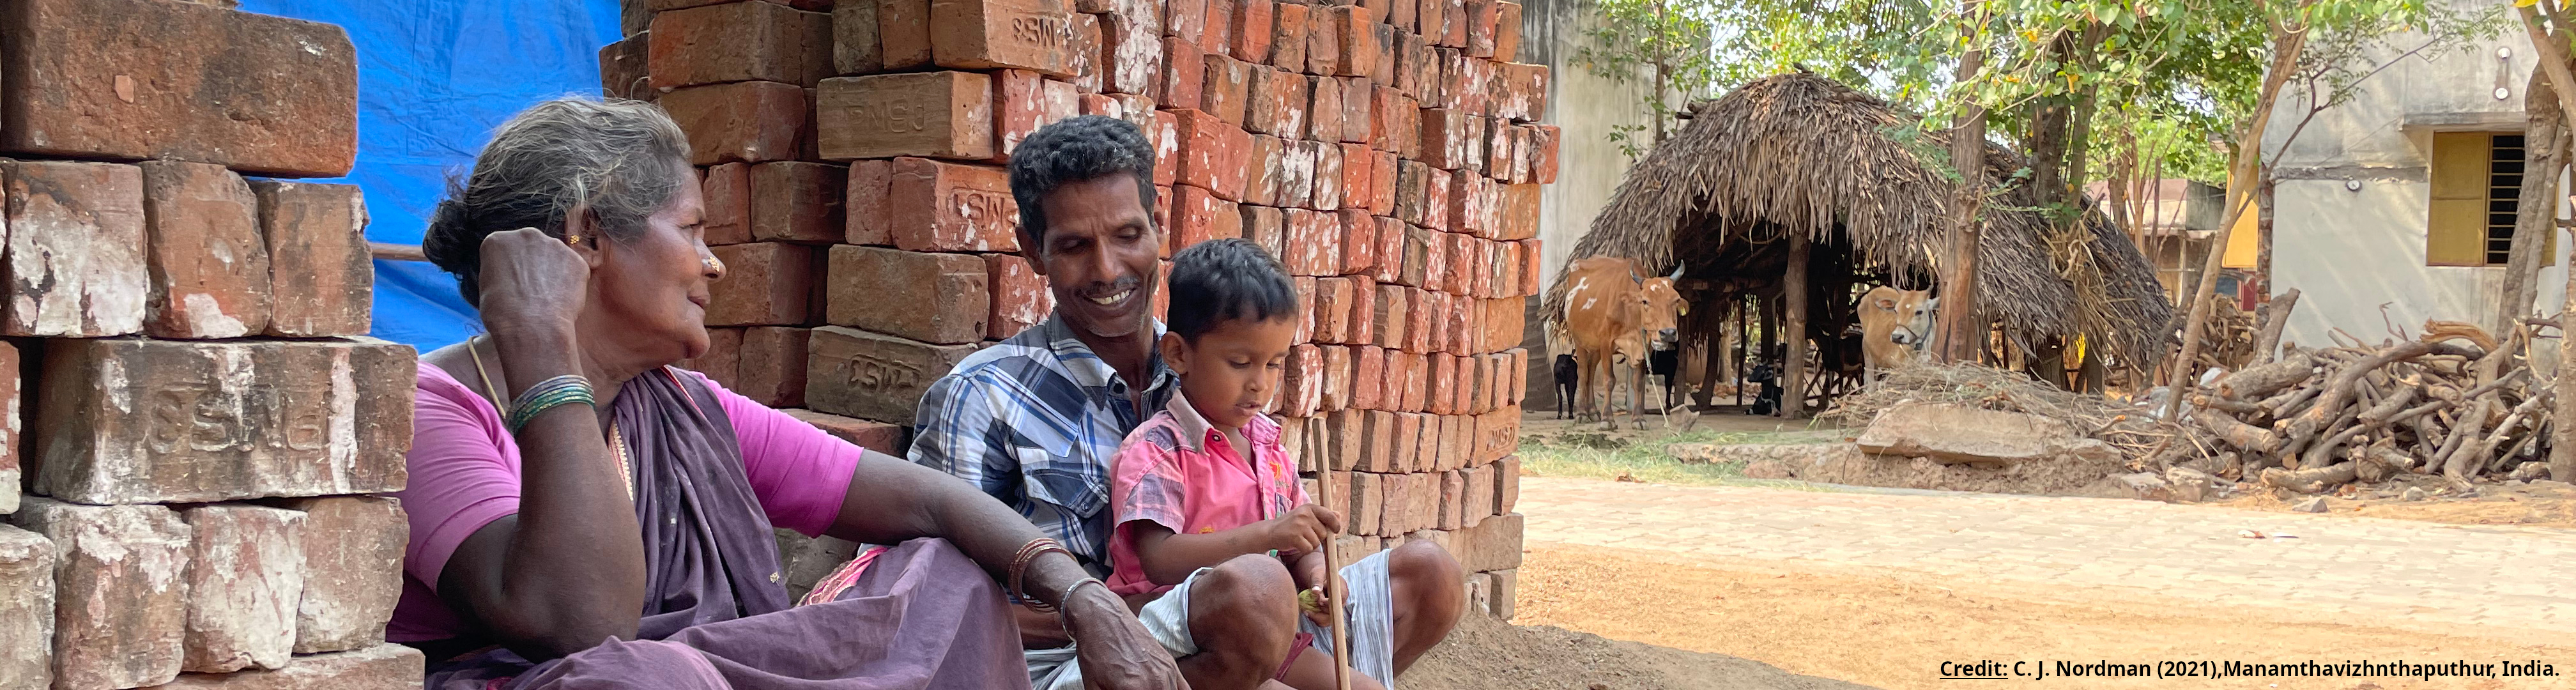
\includegraphics[width=\paperwidth]{Beamer_theme/header.jpeg}}
\renewcommand{\logoheader}{\vspace{0em}}
\renewcommand{\logoheader}{\vspace{0em}}
\renewcommand{\logofooter}{\href{https://odriis.hypotheses.org/}{\includegraphics[width=.6\linewidth]{Beamer_theme/odriis_long.jpg}}}
%\renewcommand{\logoheader}{\vspace{1.5em}}


% *****************************************************************
% Caption configuration
% *****************************************************************
\usepackage{caption}  % custom caption

\captionsetup{
font=small,
skip=1em,
labelfont={bf},
justification=centering,
singlelinecheck=false,
%textfont={bf,it},
%labelsep=endash,
%tableposition=top,
}






% *****************************************************************
% Appendix
% *****************************************************************
\usepackage{appendixnumberbeamer}
\renewcommand{\appendixname}{\texorpdfstring{\translate{appendix}}{appendix}}





% *****************************************************************
% Bibliography
% *****************************************************************

% ********** Bibtex
% \usepackage[doi, natbibapa]{apacite}
% \renewcommand\bibliographytypesize{\tiny}
% \let\realcitep\citep
% \renewcommand*{\citep}[1]{{\small\realcitep{#1}}}
% \let\realcite\cite
% \renewcommand*{\cite}[1]{{\small\realcite{#1}}}
% ********** 


% ********** Biblatex
% \usepackage[
% natbib=true,
% backend=biber,
% style=trad-abbrv,
% sorting=none, %nyt
% ]{biblatex}
% **********

% ********** Biblatex
\usepackage[
natbib=true,
backend=biber,
style=apa,
sorting=ydnt,
defernumbers=true,
citestyle=numeric,
]{biblatex}
% **********
\renewcommand*{\bibfont}{\scriptsize}





% *****************************************************************
% Bigcenter
% *****************************************************************
\makeatletter
\newskip\@bigflushglue \@bigflushglue = -100pt plus 1fil
\def\bigcenter{\trivlist \bigcentering\item\relax}
\def\bigcentering{\let\\\@centercr\rightskip\@bigflushglue%
\leftskip\@bigflushglue
\parindent\z@\parfillskip\z@skip}
\def\endbigcenter{\endtrivlist}
\makeatother






% *****************************************************************
% Box creation
% *****************************************************************
\usepackage[most]{tcolorbox}

\newtcolorbox{greenbox}[2][]{colback=ODRIISlightgreen!10,colframe=ODRIISlightgreen!10,coltitle=black,colbacktitle=ODRIISdarkgreen!20,title={#2},#1}
\newtcolorbox{brickbox}[1][]{colback=ODRIISbrick!10,colframe=ODRIISbrick!10,#1}






% *****************************************************************
% Section page
% *****************************************************************
\newcommand{\secttitle}[1]{
\begin{columns} 
\begin{column}{.4\textwidth}
\vspace*{-0mm}\hspace*{-10.1mm}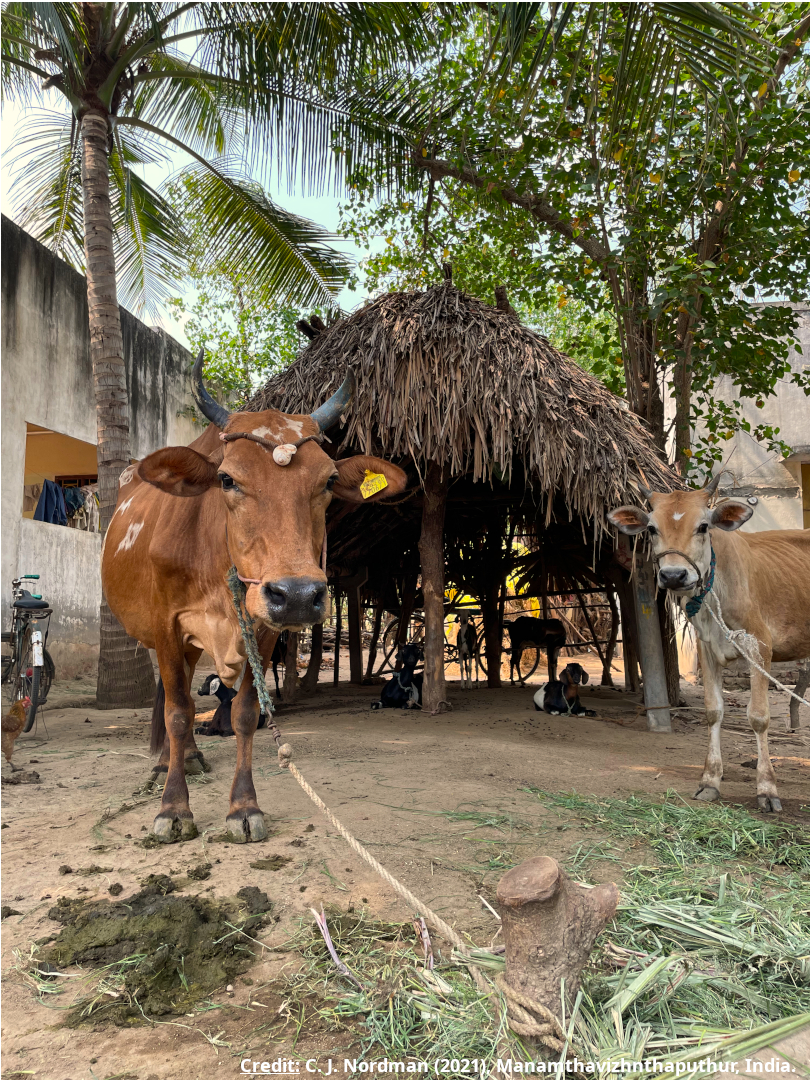
\includegraphics[height=\paperheight]{Beamer_theme/cow.jpeg}
\end{column}
\begin{column}{.6\textwidth}
\vfill
\begin{tcolorbox}[colback=ODRIISlightgreen!20,colframe=ODRIISlightgreen!20,box align=center,halign=center,valign=center]
{\LARGE \textcolor{ODRIISbrick}{#1}}
\end{tcolorbox}
\vfill
\end{column}
\end{columns}
}






% *****************************************************************
% Table
% *****************************************************************

% ********** Stars
\newcommand{\sym}[1]{\rlap{#1}}% Thanks to David Carlisle
% **********


% ********** Insert the table
\newcommand{\inserttable}[3]{
\resizebox{#3}{!}{
\begin{tabular}{#2}
\toprule
\input #1
\bottomrule
\end{tabular}
}
}
% **********


% ********** Source
\newcommand{\bottomtext}[1]{\vspace{-0ex}\captionsetup{justification=centering,font=footnotesize,singlelinecheck=false}\caption*{\hangindent=1.5em #1}}
\newcommand{\bottomnote}[1]{\bottomtext{\textit{Note}:~#1}}
\newcommand{\source}[1]{\bottomtext{\textit{Source}:~#1}}
\newcommand{\starnote}{\bottomtext{* p < 0.1, ** p < 0.05, *** p < 0.01. Standard error in parentheses.}}
% **********


% ********** siunitx config
\sisetup{
detect-mode,
tight-spacing= true,
group-digits= false ,
input-signs= ,
input-symbols= ( ) [ ] - + *,
input-open-uncertainty=,
input-close-uncertainty=,
table-align-text-post=false
}
% **********


% ********** Linebreak in cell
\newcommand{\specialcell}[2][c]{\begin{tabular}[#1]{@{}c@{}}#2\end{tabular}}
% **********


% \makeatletter
% \AddToHook{env/tabular/begin}{\let\input\@@input}
% \makeatother




% *****************************************************************
% Personnal cmd
% *****************************************************************
\newcommand{\jati}{\textit{j\={a}ti}}
\newcommand{\jatis}{\textit{j\={a}tis}}

\newcommand\dev[1]{\textbf{\textcolor{red}{#1}}}
\newcommand\res[1]{\textbf{\textcolor{ODRIISbrick}{#1}}}
\newcommand\des[1]{\textbf{\textcolor{ODRIISbrick}{#1}}}


\newcommand{\ie}{i.e.}
\newcommand{\sd}{standard deviation}
\newcommand{\pp}{percentage points}
\newcommand{\aebe}{all else being equal}
\newcommand{\Aebe}{All else being equal}
\newcommand{\ote}{other things equal}
\newcommand{\Ote}{Other things equal}
\newcommand{\cl}{confidence level}
\newcommand{\lit}{\dev{literature}}
\newcommand{\PTCS}{PT\&CS}

\newcommand{\key}[1]{\underline{\textsc{#1}}}
\newcommand{\data}[1]{\textbf{\underline{Data #1:}}~}


% ********** Symbol shortcuts
\def\@fnsymbol#1{\ensuremath{\ifcase#1\or *\or \dagger\or \ddagger\or
   \mathsection\or \mathparagraph\or \|\or **\or \dagger\dagger
   \or \ddagger\ddagger \else\@ctrerr\fi}}
   
\makeatletter
\newcommand{\ssymbol}[1]{^{\@fnsymbol{#1}}}
\makeatother
% **********


% ********** Meta
\hypersetup{
    pdftitle={State of NEEMSIS Research},
    pdfauthor={Arnaud Natal},
    pdfsubject={State of NEEMSIS Research}
}
% ********** 



% ********** Bibliography
\addbibresource{NEEMSIS.bib}
% ********** 

\setbeamercovered{transparent}

\newcommand{\red}[1]{\textcolor{red}{#1}}
\newcommand{\green}[1]{\textcolor{ODRIISdarkgreen}{#1}}

\renewcommand{\logofooter}{
\includegraphics[width=.3\linewidth]{Beamer_theme/neemsis.png}}


% *****************************************************************
% Title
% *****************************************************************
\title[NEEMSIS State of Research]{\textsc{State of 
\includegraphics[height=1.5em]{Beamer_theme/neemsis} Research}}
\author[A. Natal]{\href{https://neemsis.hypotheses.org/team/arnaud-natal}{\textcolor{ODRIISdarkgreen}{Arnaud Natal}} \small\textcolor{ODRIISlightgreen}{University of Bordeaux and IFP}}
\institute{\\ \small September, 2025 \\ \scriptsize \href{https://neemsis.hypotheses.org/}{\textcolor{ODRIISbrick}{https://neemsis.hypotheses.org/}}} 

% ******************************************************************
\begin{document}

\maketitle




% *******************
\section*{Foreword}
\begin{frame}{Foreword}
\begin{small}


This PDF document provides an overview of the research undertaken using the original \href{https://neemsis.hypotheses.org}{\textit{Network, Employment, dEbt, Mobility, and Skills in South India Survey}} (NEEMSIS).

\begin{brickbox}
NEEMSIS is a longitudinal data collection tool that aims at understanding the links between labour, skills, financial practices, social and migration dynamics and social networks formation in rural Tamil Nadu, India, through individual and household surveys.  NEEMSIS is based on the baseline survey RUME (\href{https://odriis.hypotheses.org/rume}{\textit{RUral Microfinance and Employment}}) conducted in 2010. NEEMSIS has so far been conducted in 2016–2017 and 2020–2021 among more than 600 households. A third wave of NEEMSIS is planned for 2025-2026 (which will constitute a panel with four points in time between 2010 and 2025-2026). \\
These data collections are carried out within the framework of the \href{https://odriis.hypotheses.org/}{
\includegraphics[height=2em]{Beamer_theme/odriis}}. See \href{https://odriis.hypotheses.org/}{https://odriis.hypotheses.org/}
\end{brickbox}

\end{small}
\end{frame}
% *******************



% *******************
\section*{Introduction}
\begin{frame}[plain,noframenumbering]
\label{introduction}

\secttitle{1. Introduction}

\end{frame}
% *******************



% *******************
\begin{frame}{Study area}

\begin{figure}[h]
\centering
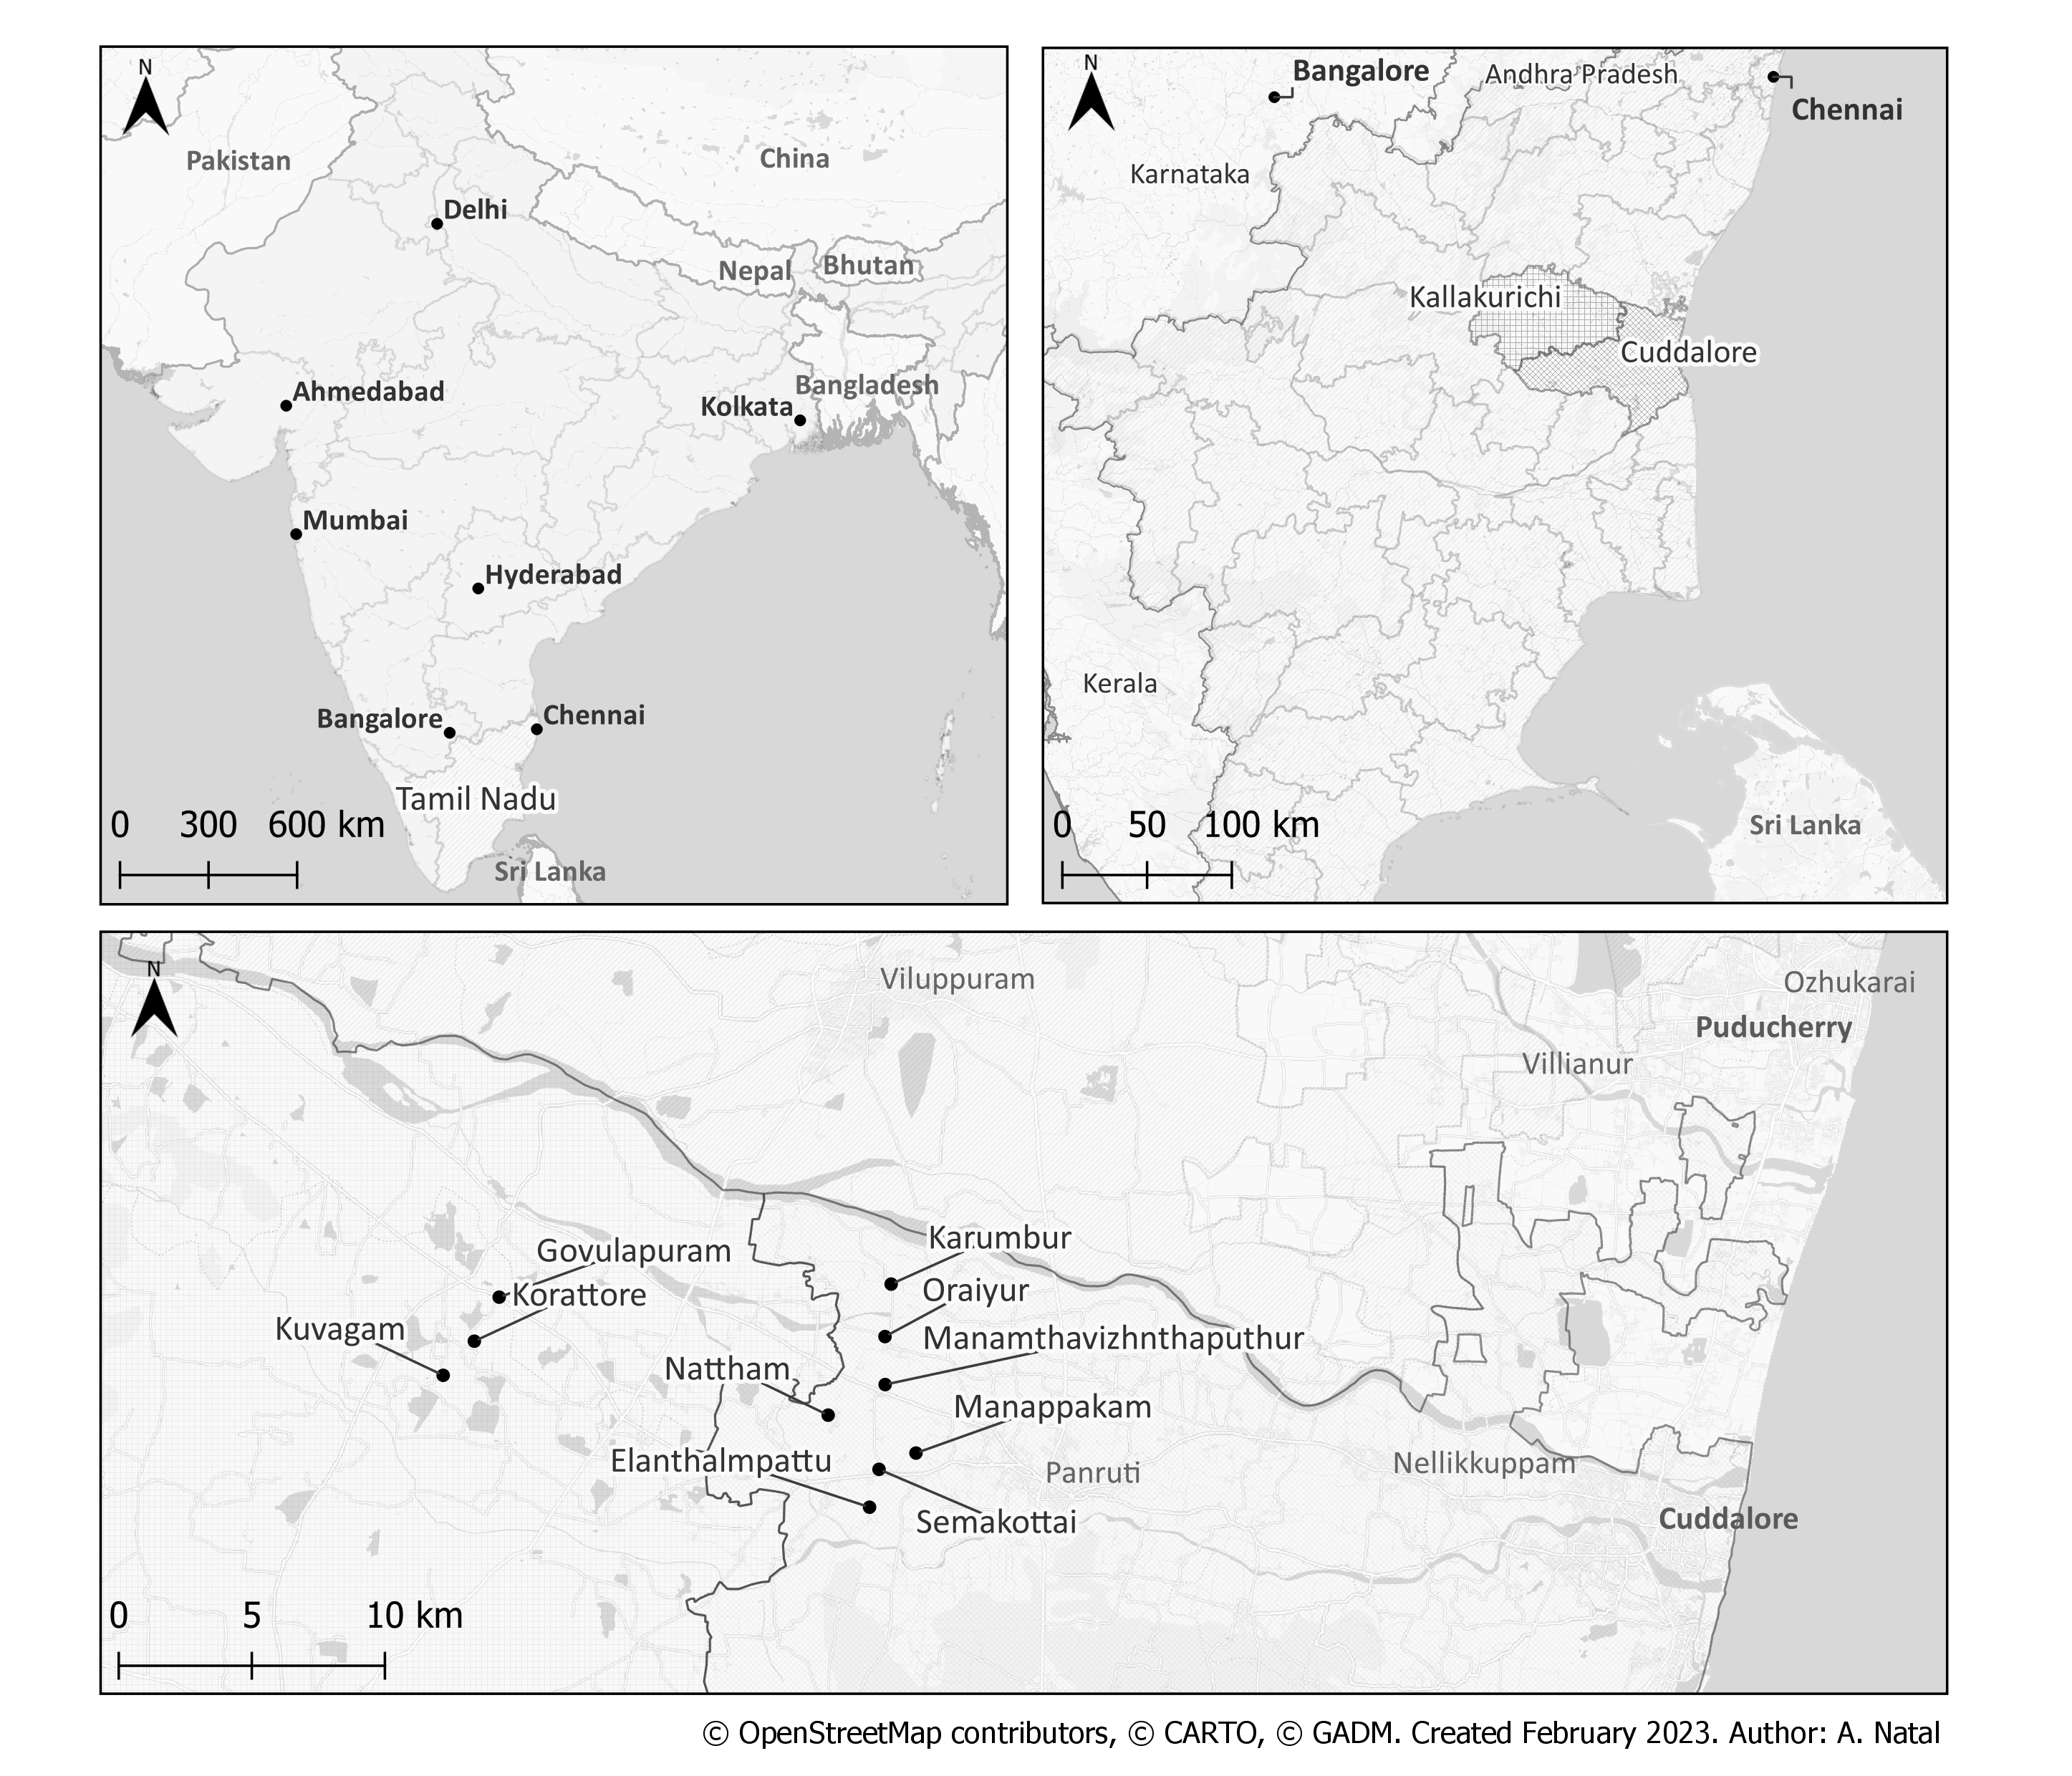
\includegraphics[width=0.5\columnwidth]{INPUT/RUME-NEEMSIS.png}
\end{figure}

\end{frame}
% *******************



% *******************
\begin{frame}{Core teams}
\begin{scriptsize}

\begin{table}[h]
  \centering
    \begin{tabular}{llll}
    \toprule
    RUME  & NEEMSIS-1 & NEEMSIS-2 & NEEMSIS-3 \\
    \midrule
    I. Guérin & C. J. Nordman & C. J. Nordman & C. J. Nordman \\
    G. Venkat & G. Venkat & G. Venkat & G. Venkat \\
    M. Roesch & I. Guérin & I. Guérin & I. Guérin \\
    S. Michiels & S. Michiels & S. Michiels & S. Michiels \\
    A. Raj & Y. Lanos & C. Mouchel & C. Mouchel \\
          & A. Hilger & A. Natal & A. Natal \\
          & S. Kumar & M. Di Santolo & M. Di Santolo \\
          & A. Raj & A. Hilger & F. Desplanques \\
          &       & A. Raj & A. Raj \\
    \bottomrule
    \end{tabular}%
\end{table}%

\end{scriptsize}
\end{frame}
% *******************




% *******************
\begin{frame}{Ressources 1}
\begin{small}

For further details on the NEEMSIS longitudinal survey: 

\begin{center}
\href{https://neemsis.hypotheses.org/}{https://neemsis.hypotheses.org/}
\end{center}
\begin{figure}[h]
\centering
\href{https://neemsis.hypotheses.org/}{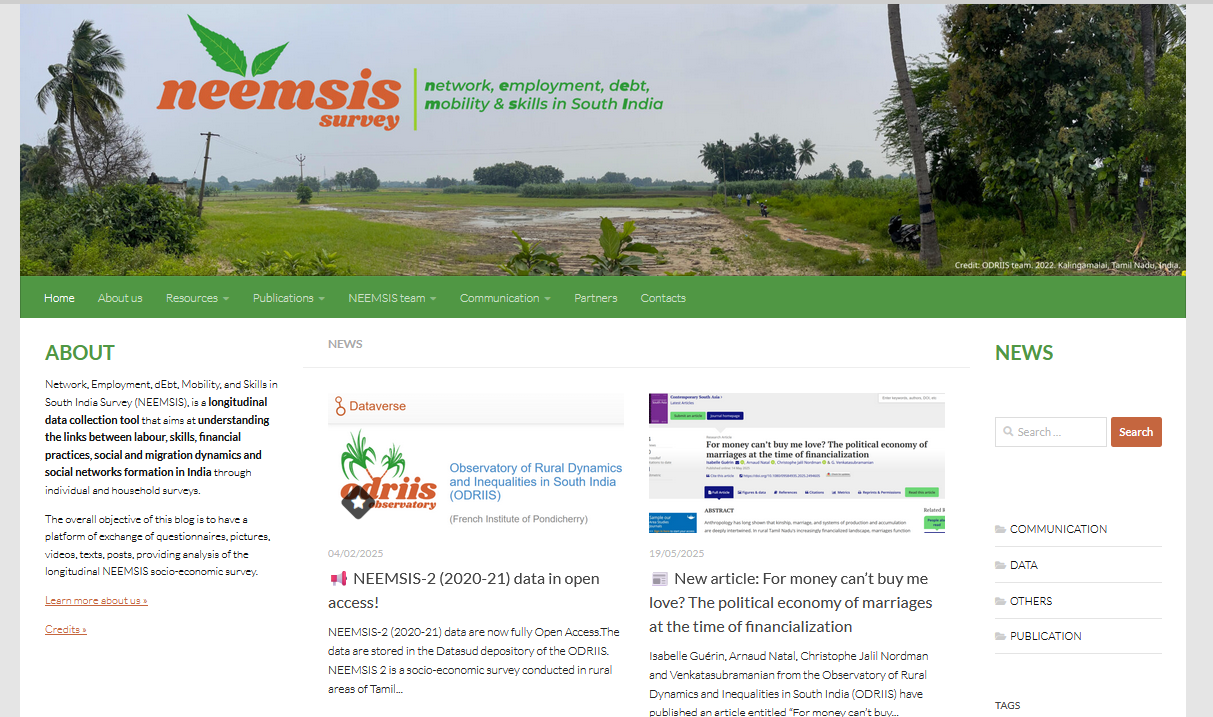
\includegraphics[width=0.5\columnwidth]{INPUT/website.png}}
\end{figure}

\end{small}
\end{frame}
% *******************




% *******************
\begin{frame}{Ressources 2}
\begin{scriptsize}

\begin{greenbox}{Article presenting the data}
Nordman, C. J., Venkatasubramanian, G., Guérin, I., Natal, A., Mouchel, C., Michiels, S., \& Di Santolo, M. (2025). Networks, Employment, Debt, Mobilities, and Skills in India Survey (NEEMSIS): Presentation of a longitudinal data collection tool. \textit{Population, 80}(1).
\end{greenbox}

\begin{greenbox}{Article presenting the trends observed in the data between 2010 and 2020-2021}
Di Santolo, M., Guérin, I., Michiels, S., Mouchel, C., Natal, A., Nordman, C. J., \& Venkatasubramanian, G. (2024). A Decade in Rural Tamil Nadu: Socio-Economic, Labour and Migration Trends from an Original Longitudinal Household Survey. \textit{Economic \& Political Weekly, 59}(43), 62–71.
\end{greenbox}

\begin{greenbox}{The video presentation of the survey}
\textit{Making of the NEEMSIS Survey} available at \href{https://www.youtube.com/watch?v=b68yu1CTW0U}{https://www.youtube.com/watch?v=b68yu1CTW0U}
\end{greenbox}


\end{scriptsize}
\end{frame}
% *******************




% *******************
\begin{frame}{Framework of this document}
\label{framework}
\begin{small}

\begin{figure}[h]
\centering
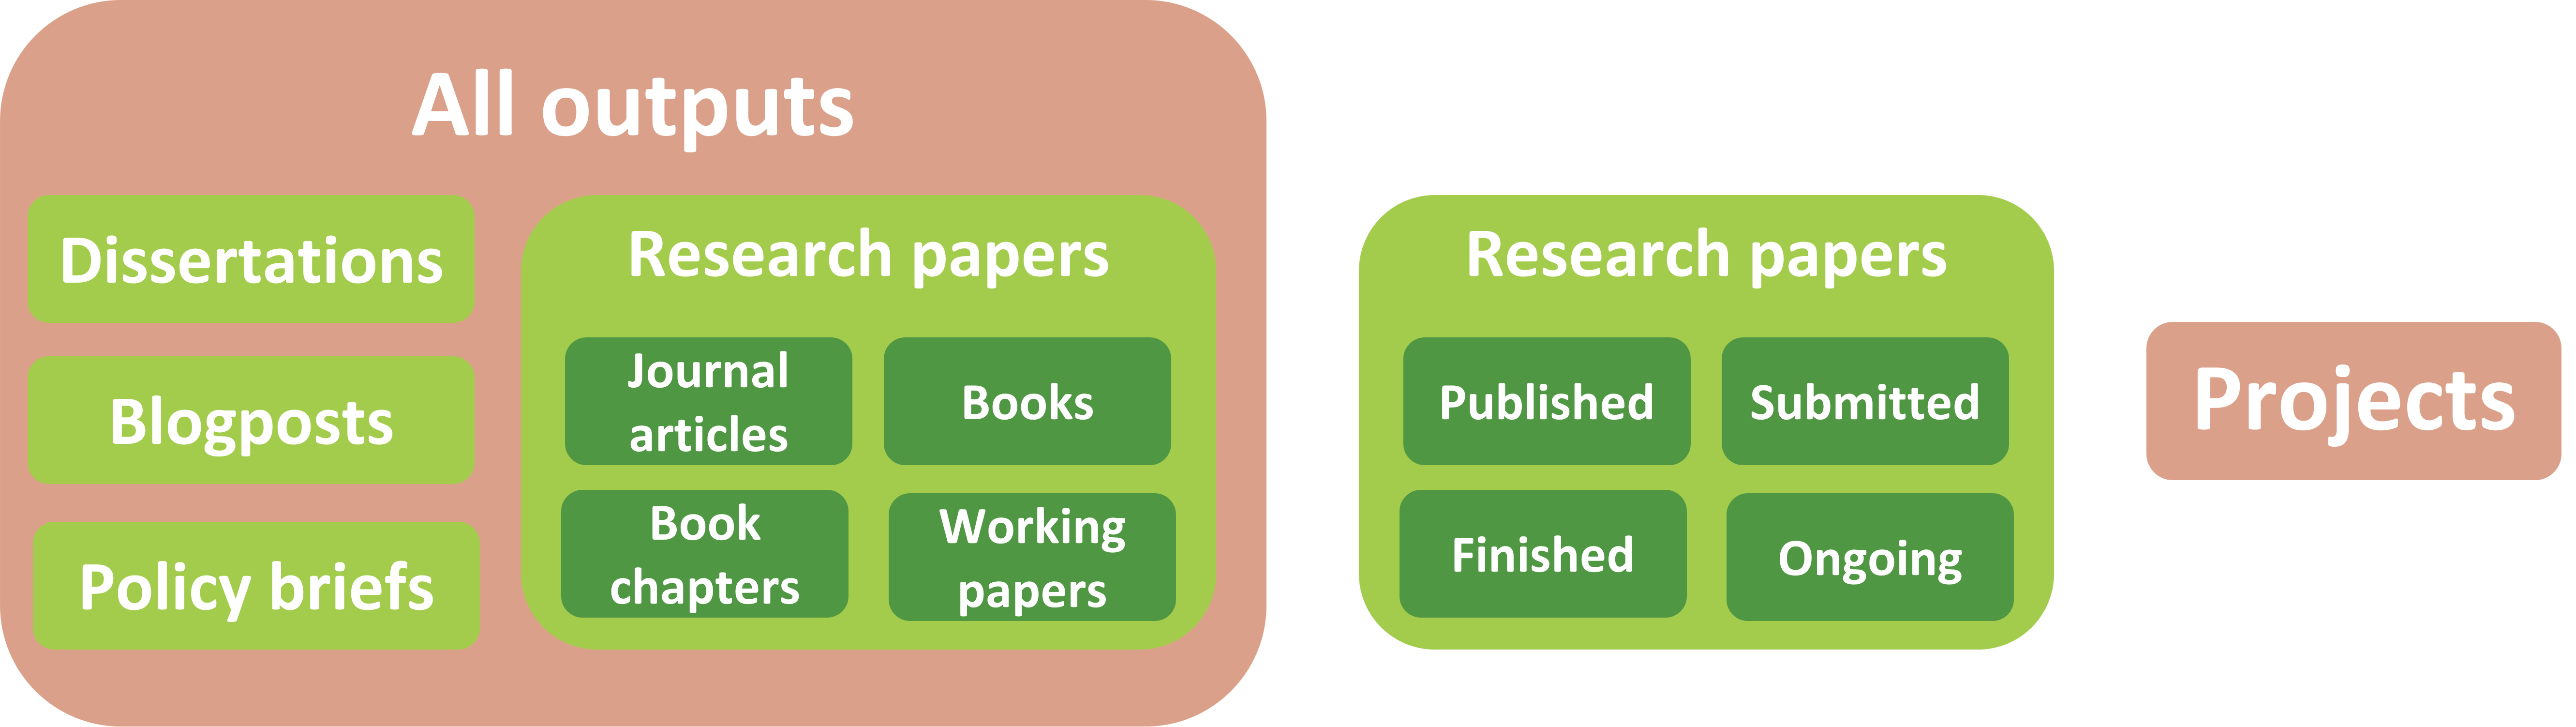
\includegraphics[width=0.7\columnwidth]{INPUT/diagram.png}
\end{figure}

All of the above terms are defined in the appendix. \hyperlink{appendix}{\beamerbutton{See »}}

Research papers are sometimes classified according to their type (journal, book, etc.) and status (published, submitted, etc.).

\begin{scriptsize}
\begin{greenbox}{Example}
Journal articles are either published, submitted, or ongoing. And, published articles include articles in journals, books, and chapters.
\end{greenbox}
\end{scriptsize}

\end{small}
\end{frame}
% *******************





% *******************
\begin{frame}{A brief overview}
\begin{scriptsize}

\begin{brickbox}
* Few researchers have requested access to the data. \\
* 46 outputs were produced, including 16 journal articles, 1 book and 6 dissertations. \\
* Among the research papers, 50\% are cross-sectional and 50\% are longitudinal. \\
* Debt is the most common topic (60\% of the papers), then employment (30\%), and gender (25\%). \\
* Nordman is the most prolific (64\% of research papers), then Guérin (50\%), and Natal/Venkat (42\%). \\
* 5 papers are currently submitted, 4 are ongoing and 7 are in project. \\
* All published papers using RUME and NEEMSIS data account for 430 citations. \\
* The most cited article is ``Debt in Rural South India'' (2013, \textit{The Journal of Development Studies}). \\
* Guérin is the most cited researcher.
\end{brickbox}

\end{scriptsize}
\end{frame}
% *******************




% *******************
\begin{frame}{Plan}
\begin{scriptsize}

\begin{enumerate}
\item Introduction \hyperlink{introduction}{\beamerbutton{See »}}
\item Data access request \hyperlink{data}{\beamerbutton{See »}}
\item All outputs \hyperlink{all}{\beamerbutton{See »}}
\item Research papers \hyperlink{research}{\beamerbutton{See »}}
\item Published papers \hyperlink{published}{\beamerbutton{See »}}
\item In details (journals, dissertations, blog posts) \hyperlink{details}{\beamerbutton{See »}}
\item Upcoming papers (submitted, ongoing, projects) \hyperlink{upcoming}{\beamerbutton{See »}}
\item Conclusion \hyperlink{conclusion}{\beamerbutton{See »}}
\item References \hyperlink{references}{\beamerbutton{See »}}
\end{enumerate}

\begin{brickbox}
For an overview of how these concepts fit together, see the framework. \hyperlink{framework}{\beamerbutton{See »}}
\end{brickbox}

\end{scriptsize}
\end{frame}
% *******************





% *******************
\section*{Data access request}
\begin{frame}[plain,noframenumbering]
\label{data}

\secttitle{2. Data access request}

\end{frame}
% *******************





% *******************
\begin{frame}{Data access request}
\begin{small}

Data are freely available on DataSuds: \href{https://dataverse.ird.fr/dataverse/odriis}{https://dataverse.ird.fr/dataverse/odriis}

\begin{table}[]
\begin{tabular}{lcc}
\toprule
Data*     & Before 2025 & Since 2025** \\
\midrule
RUME      & 7             & 0          \\
NEEMSIS-1 & 5             & 1          \\
NEEMSIS-2 & 0             & 3          \\
\bottomrule
\end{tabular}
\end{table}

\begin{scriptsize}
\begin{brickbox}
*Household data is the master database. Other shared databases (e.g., loans, occupations, etc.) must always be associated with the household database. That is why only requests for household bases are reported here. \\
**Since January 2025, access to data requires that: (i) the applicant complete a data use agreement; (ii) the request be validated by the survey manager.
\end{brickbox}
\end{scriptsize}

\end{small}
\end{frame}
% *******************







% *******************
\section*{All outputs}
\begin{frame}[plain,noframenumbering]
\label{all}

\secttitle{3. All outputs}

\end{frame}
% *******************





% *******************
\begin{frame}{All ouputs}

\begin{figure}[h]
\centering
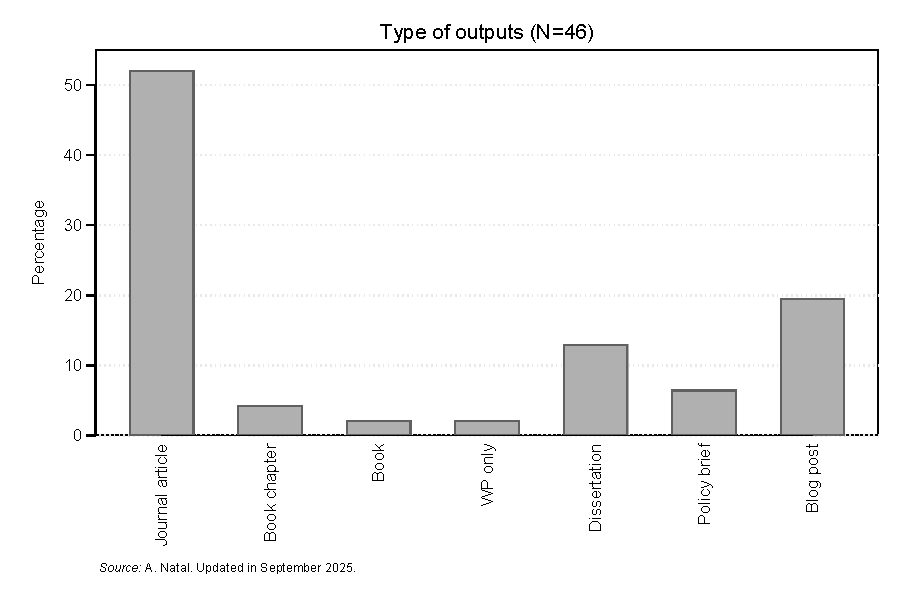
\includegraphics[width=0.7\columnwidth]{INPUT/A_type}
\end{figure}

\end{frame}
% *******************






% *******************
\section*{Research papers}
\begin{frame}[plain,noframenumbering]
\label{research}

\secttitle{4. Research papers}

\end{frame}
% *******************





% *******************
\begin{frame}{Research papers 1}

\begin{figure}[h]
\centering
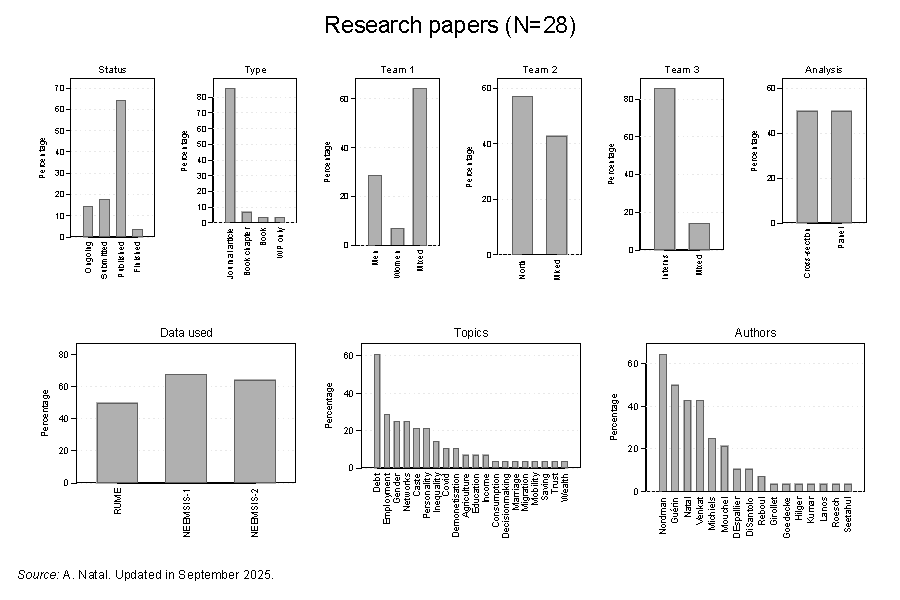
\includegraphics[width=0.7\columnwidth]{INPUT/RP_global}
\end{figure}

\end{frame}
% *******************




% *******************
\begin{frame}{Research papers 2}

\begin{figure}[h]
\centering
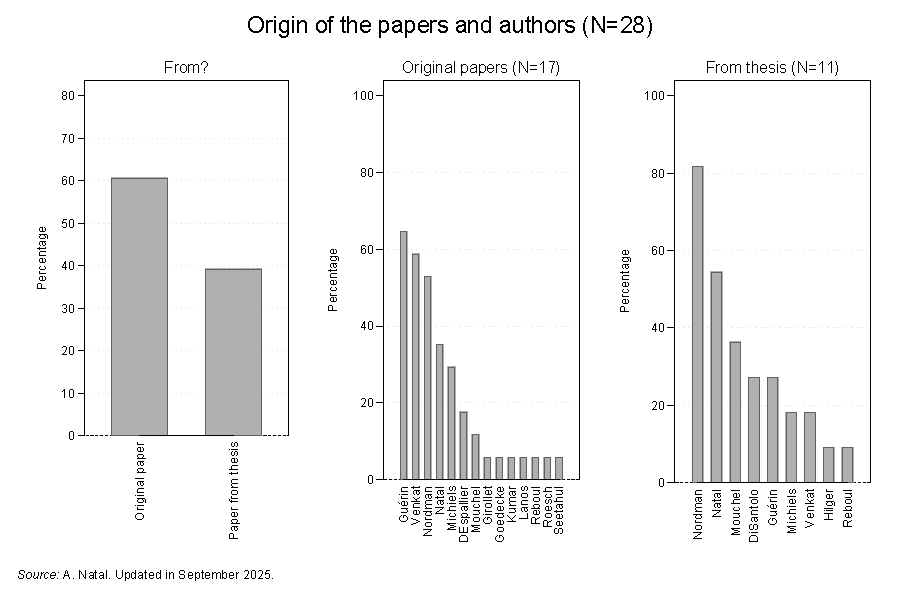
\includegraphics[width=0.7\columnwidth]{INPUT/RP_origins}
\end{figure}

\end{frame}
% *******************



% *******************
\begin{frame}{Research papers 3}

\begin{figure}[h]
\centering
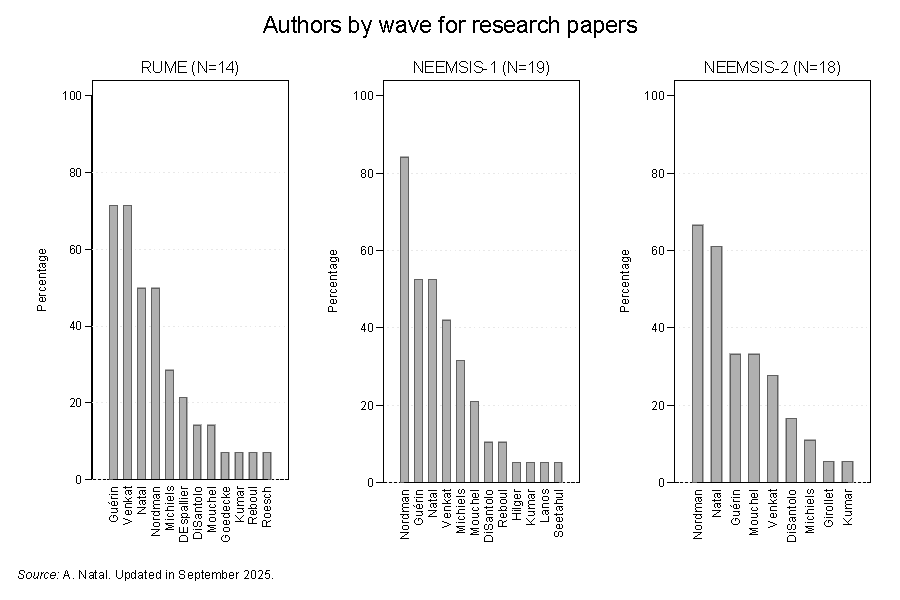
\includegraphics[width=0.7\columnwidth]{INPUT/RP_authorswave}
\end{figure}

\end{frame}
% *******************






% *******************
\begin{frame}{Research papers 4}

\begin{figure}[h]
\centering
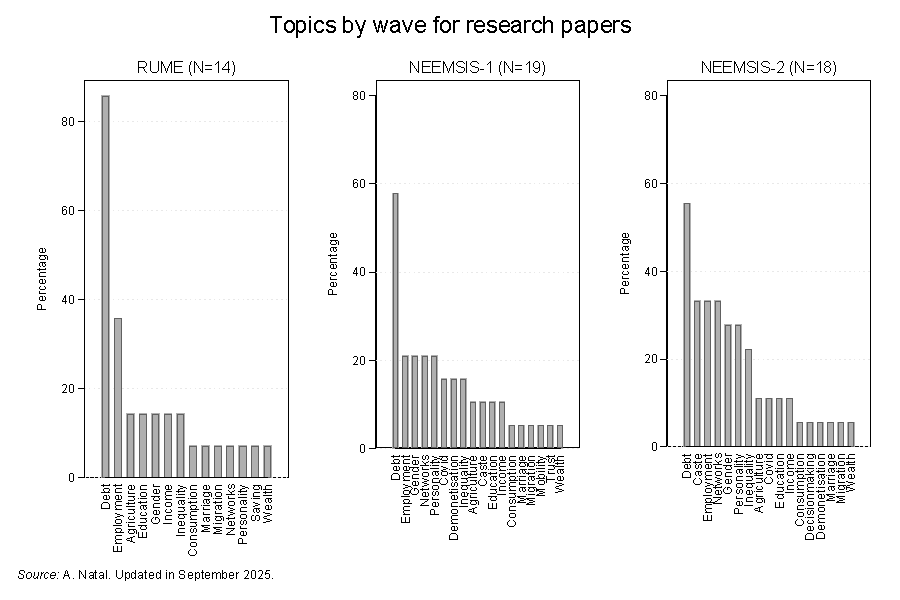
\includegraphics[width=0.7\columnwidth]{INPUT/RP_topicswave}
\end{figure}

\end{frame}
% *******************




% *******************
\begin{frame}{Research papers 5}
\begin{footnotesize}

Word cloud on RUME paper abstracts
\begin{figure}[h]
\centering
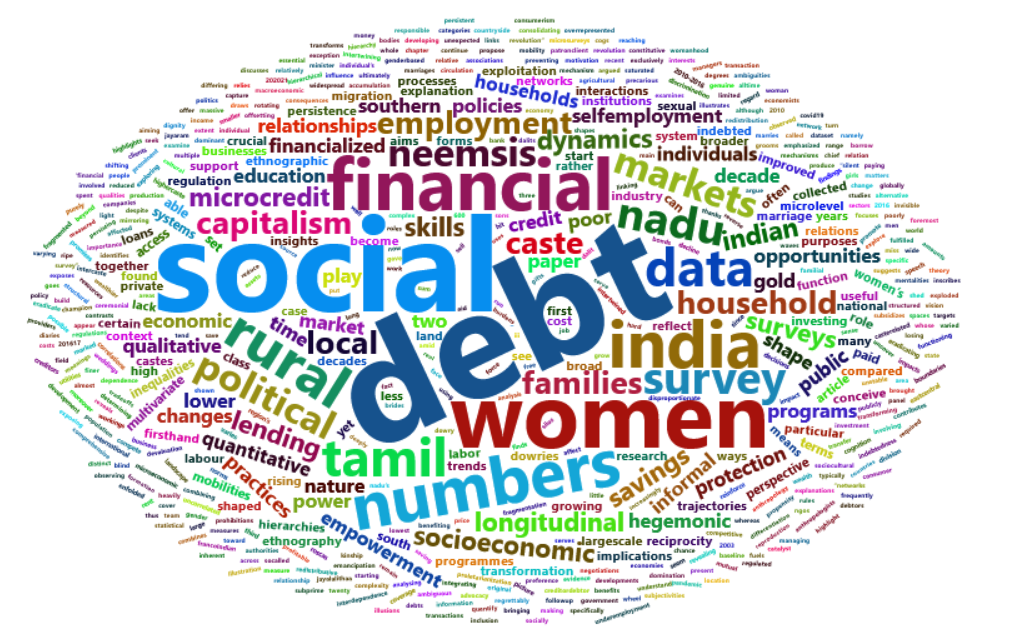
\includegraphics[width=0.6\columnwidth]{INPUT/rume.png}
\end{figure}
\textit{Source:} A. Natal. Updated in September 2025.

\end{footnotesize}
\end{frame}
% *******************




% *******************
\begin{frame}{Research papers 6}
\begin{footnotesize}

Word cloud on NEEMSIS-1 paper abstracts
\begin{figure}[h]
\centering
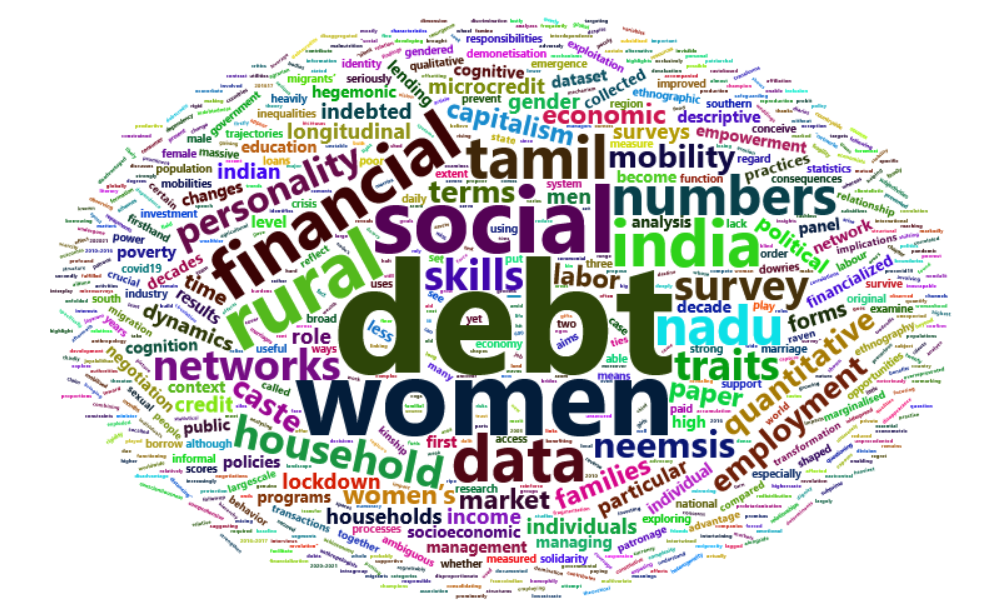
\includegraphics[width=0.65\columnwidth]{INPUT/neemsis1.png}
\end{figure}
\textit{Source:} A. Natal. Updated in September 2025.

\end{footnotesize}
\end{frame}
% *******************



% *******************
\begin{frame}{Research papers 7}
\begin{footnotesize}

Word cloud on NEEMSIS-2 paper abstracts
\begin{figure}[h]
\centering
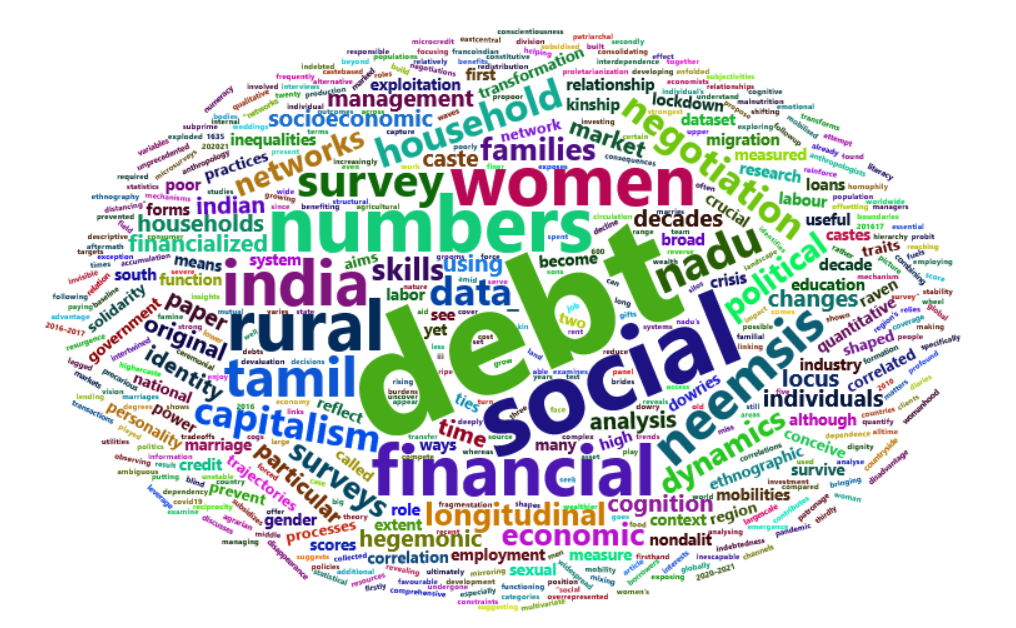
\includegraphics[width=0.65\columnwidth]{INPUT/neemsis2.png}
\end{figure}
\textit{Source:} A. Natal. Updated in September 2025.

\end{footnotesize}
\end{frame}
% *******************







% *******************
\section*{Published papers}
\begin{frame}[plain,noframenumbering]
\label{published}

\secttitle{5. Published papers}

\end{frame}
% *******************





% *******************
\begin{frame}{Published papers 1}

\begin{figure}[h]
\centering
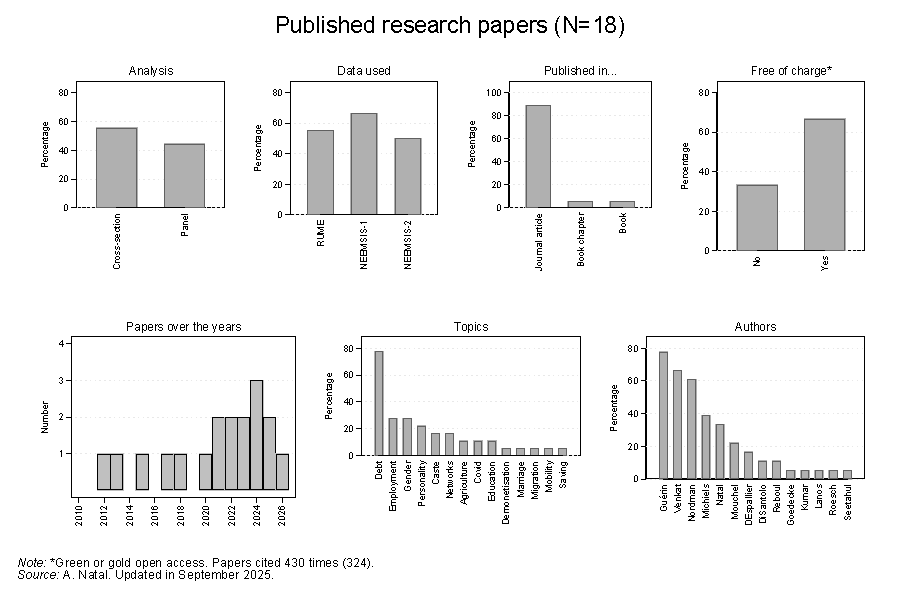
\includegraphics[width=0.7\columnwidth]{INPUT/PP_global}
\end{figure}

\end{frame}
% *******************






% *******************
\begin{frame}{Published papers 2}

\begin{figure}[h]
\centering
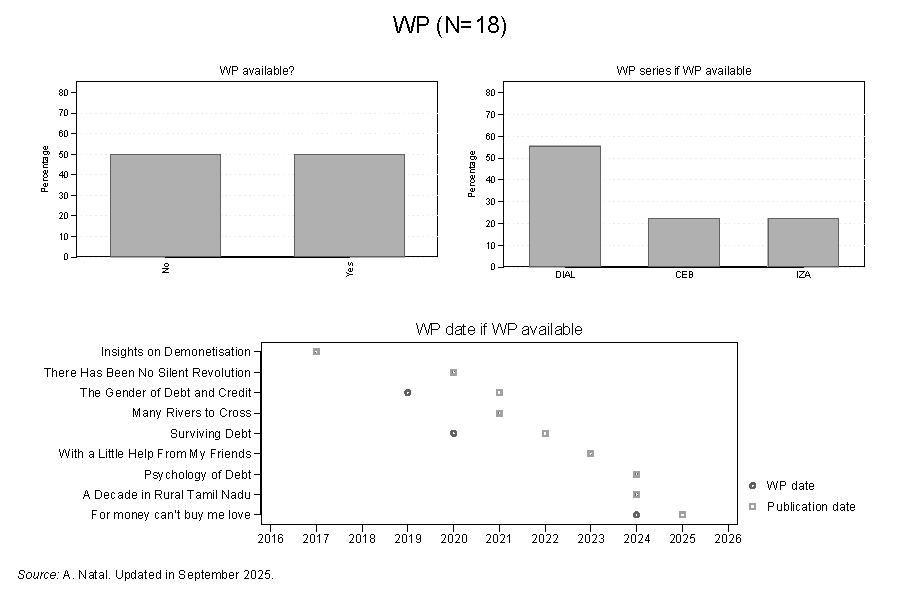
\includegraphics[width=0.7\columnwidth]{INPUT/PP_wp}
\end{figure}

\end{frame}
% *******************






% *******************
\begin{frame}{Published papers 3}

\begin{figure}[h]
\centering
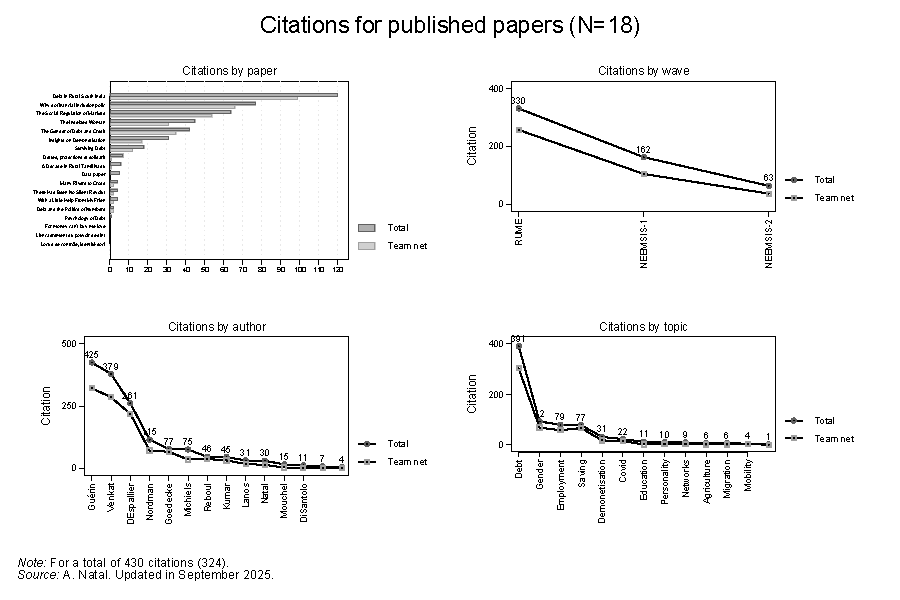
\includegraphics[width=0.7\columnwidth]{INPUT/PP_citations}
\end{figure}

\end{frame}
% *******************








% *******************
\section*{In details}
\begin{frame}[plain,noframenumbering]
\label{details}

\secttitle{6. In details}

\end{frame}
% *******************





% *******************
\begin{frame}{Journals}

\begin{figure}[h]
\centering
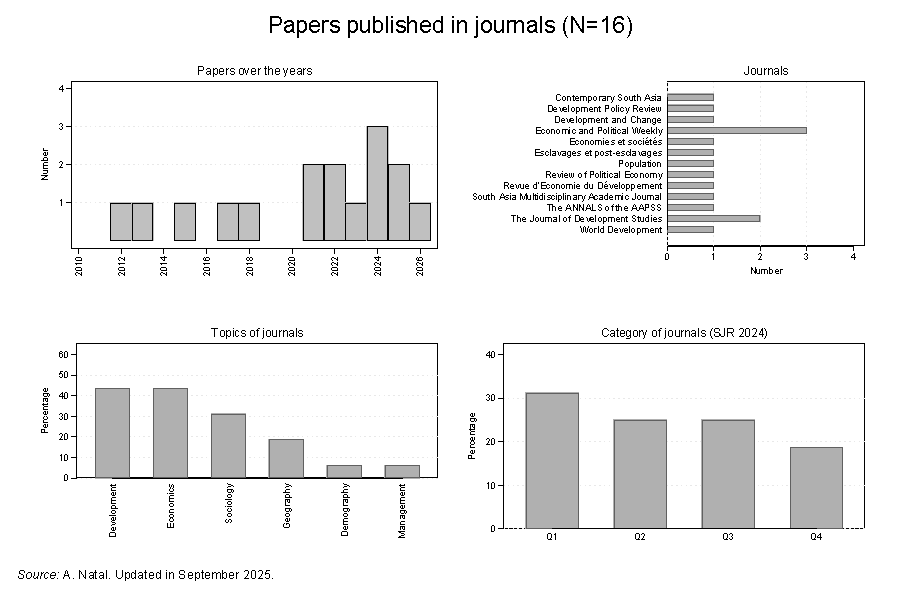
\includegraphics[width=0.7\columnwidth]{INPUT/J_global}
\end{figure}

\end{frame}
% *******************





% *******************
\begin{frame}{Dissertations}

\begin{figure}[h]
\centering
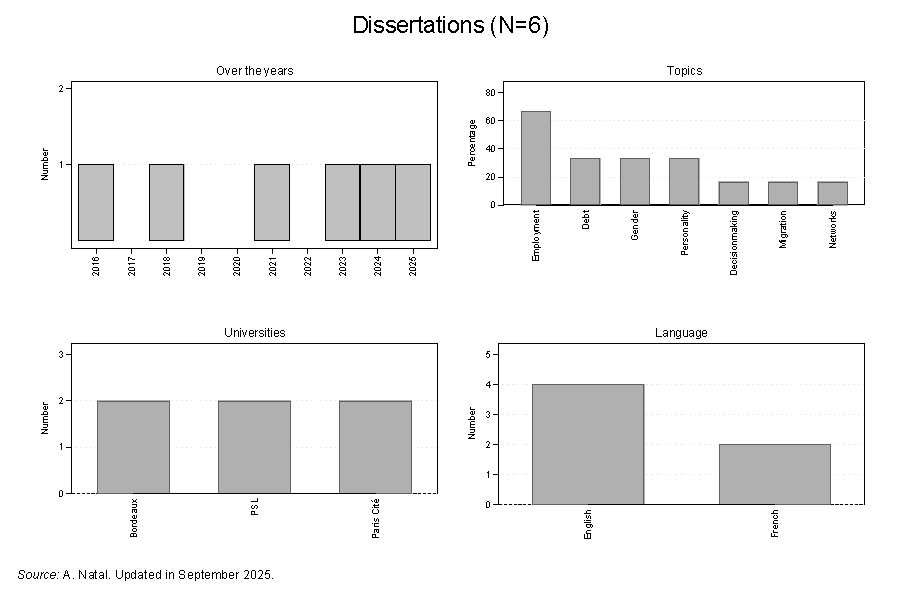
\includegraphics[width=0.7\columnwidth]{INPUT/D_global}
\end{figure}

\end{frame}
% *******************





% *******************
\begin{frame}{Blog posts}

\begin{figure}[h]
\centering
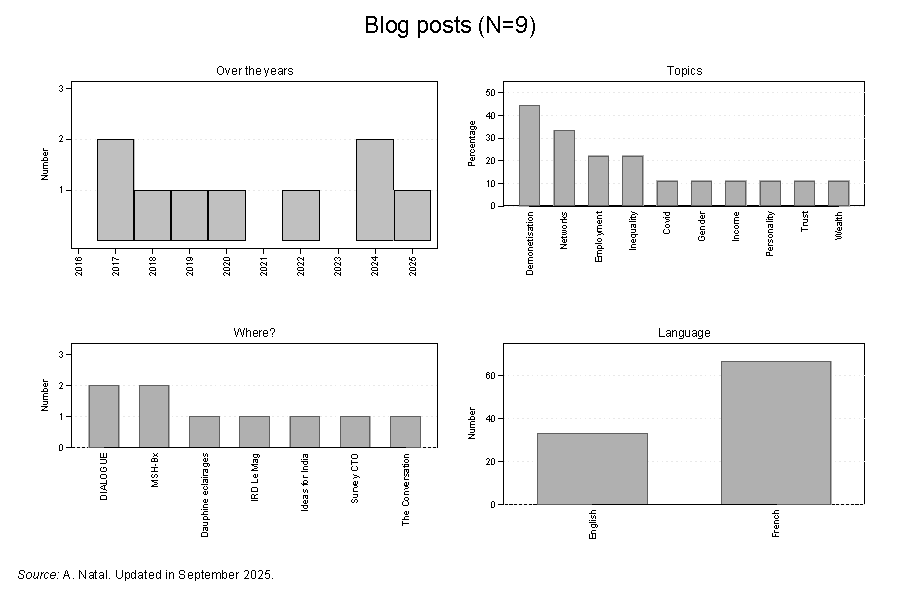
\includegraphics[width=0.7\columnwidth]{INPUT/BP_global}
\end{figure}

\end{frame}
% *******************





% *******************
\section*{Upcoming papers}
\begin{frame}[plain,noframenumbering]
\label{upcoming}

\secttitle{7. Upcoming papers}

\end{frame}
% *******************




% *******************
\begin{frame}{Submitted}

\begin{figure}[h]
\centering
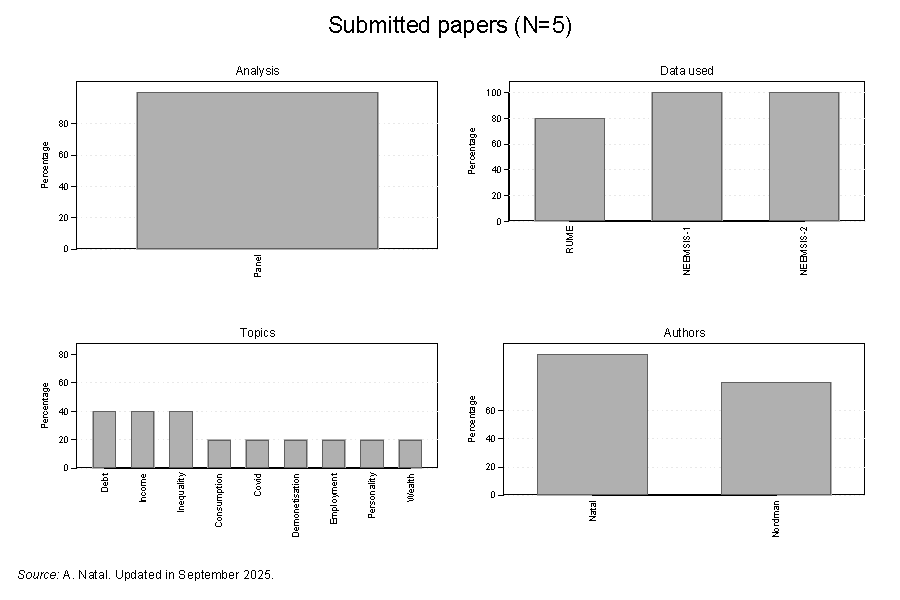
\includegraphics[width=0.7\columnwidth]{INPUT/SU_global}
\end{figure}

\end{frame}
% *******************





% *******************
\begin{frame}{Ongoing}

\begin{figure}[h]
\centering
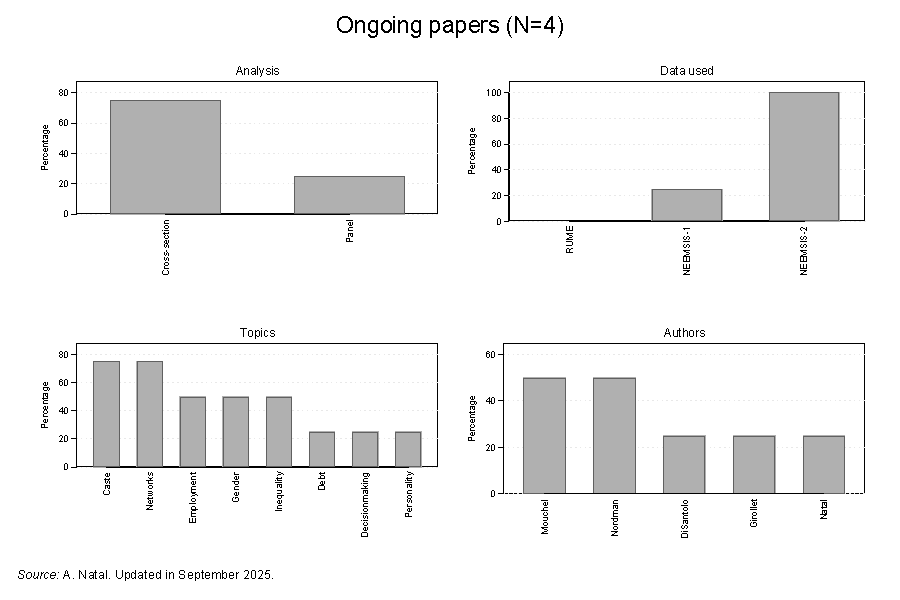
\includegraphics[width=0.7\columnwidth]{INPUT/OG_global}
\end{figure}

\end{frame}
% *******************




% *******************
\begin{frame}{Projects 1}
\begin{scriptsize}

\begin{greenbox}{\textit{The curse of having a job. Threats on female employment in a context of rising patriarcal norms}}
Using NEEMSIS-2, Di Santolo, Guérin, and Mouchel (corresponding author) want to...
\end{greenbox}

\begin{greenbox}{\textit{Intra-household inequality and recourse to debt}}
Using NEEMSIS-3, Di Santolo and Natal (corresponding author) want to study the effects of intra-household inequalities in consumption and income on household/individual debt (recourse, burden).
\end{greenbox}

\begin{greenbox}{\textit{The Ties That Bind: Lender-Borrower Relationships and Indebtedness in Rural South India}}
Using NEEMSIS-2, Girollet and Natal (corresponding author) want to study the effects of lender-borrower relationships on loan characteristics (price, repayment difficulties, services associated with loans).
\end{greenbox}


\end{scriptsize}
\end{frame}
% *******************





% *******************
\begin{frame}{Projects 2}
\begin{scriptsize}

\begin{greenbox}{\textit{The Role of Networks in Labor Market Segmentation}}
Using NEEMSIS-2, Mouchel (corresponding author) wants to...
\end{greenbox}

\begin{greenbox}{\textit{The Financial Burden of Education in Rural South India}}
Using NEEMSIS-3, Natal (corresponding author) wants to study the financialisation/commodification of education: How much does education cost? How do families finance it? What are the effects on family debt? What are the effects in terms of well-being? \\
\underline{Collaboration:} Guérin, Nordman?
\end{greenbox}

\begin{greenbox}{\textit{Stability Over Time of the Locus of Control}}
Using NEEMSIS-2 and NEEMSIS-3, in a short paper, Natal (corresponding author) wants to examine the stability of the locus of control over time. Conduct regressions to examine the explanatory factors of change. Possibly conduct a PSM with the effects of COVID. \\
\underline{Collaboration:} Nordman?
\end{greenbox}


\end{scriptsize}
\end{frame}
% *******************






% *******************
\begin{frame}{Projects 3}
\begin{scriptsize}

\begin{greenbox}{\textit{Household Indebtedness Landscape: Evolution between 2010 and 2025}}
Using RUME to NEEMSIS-3, Natal (corresponding author) wants to conduct a loan-level MCA to look at the transformation of debt practices since 2010. Try to extract household-level variables to do econometrics and look at the determinants of financial vulnerability. \\
\underline{Collaboration:} Guérin, Michiels?
\end{greenbox}

\end{scriptsize}
\end{frame}
% *******************



% *******************
\section*{Conclusion}
\begin{frame}[plain,noframenumbering]
\label{conclusion}

\secttitle{8. Conclusion}

\end{frame}
% *******************


% *******************
\begin{frame}{Conclusion}
\begin{small}

\begin{brickbox}
* Few researchers have requested access to the data. \\
* 46 ouputs were produced, including 16 journal articles, 1 book and 6 dissertations. \\
* Debt is the most common topic (60\% of the papers), then employment (30\%), and gender (25\%). \\
* All published papers using RUME and NEEMSIS data account for 430 citations. \\
* 5 papers are currently submitted, 4 are ongoing and 7 are in project.	
\end{brickbox}

\vspace*{3em}
Topics such as \textbf{Agriculture}, \textbf{Migration}, and \textbf{Education} have been understudied and \underline{should be studied in the future}.

\end{small}
\end{frame}
% *******************




% *******************
\section*{References}
\begin{frame}[plain,noframenumbering]
\label{references}

\secttitle{9. References}

\end{frame}
% *******************



% *******************
\begin{frame}[noframenumbering, allowframebreaks]{Published papers}

\printbibliography[keyword={published},heading=none,resetnumbers=true]

\end{frame}
% *******************


% *******************
\begin{frame}[noframenumbering, allowframebreaks]{Unpublished working papers}

\printbibliography[keyword={WP},heading=none,resetnumbers=true]

\end{frame}
% *******************

% *******************
\begin{frame}[noframenumbering, allowframebreaks]{Dissertations}

\printbibliography[keyword={dissertation},heading=none,resetnumbers=true]

\end{frame}
% *******************


% *******************
\begin{frame}[noframenumbering, allowframebreaks]{Policy briefs}

\printbibliography[keyword={PB},heading=none,resetnumbers=true]

\end{frame}
% *******************


% *******************
\begin{frame}[noframenumbering, allowframebreaks]{Blog posts}

\printbibliography[keyword={BP},heading=none,resetnumbers=true]

\end{frame}
% *******************


% *******************
\begin{frame}[noframenumbering, allowframebreaks]{Submitted}

\printbibliography[keyword={Sub},heading=none,resetnumbers=true]

\end{frame}
% *******************


% *******************
\begin{frame}[noframenumbering, allowframebreaks]{Ongoing}

\printbibliography[keyword={On},heading=none,resetnumbers=true]

\end{frame}
% *******************


% *******************
\begin{frame}[noframenumbering, allowframebreaks]{Projects}

\printbibliography[keyword={project},heading=none,resetnumbers=true]

\end{frame}
% *******************





% *******************
\section*{Appendix}
\begin{frame}[plain,noframenumbering]

\secttitle{Appendix}

\end{frame}
% *******************



% *******************
\begin{frame}[noframenumbering]{Definitions}
\begin{scriptsize}

\textbf{Journal articles:} Articles published in journals.

\textbf{Book chapters:} Articles published in books.

\textbf{Books:} Published books.

\textbf{Working papers (WP):} Completed articles that remained at the working paper stage (not published in journals or books).

\textbf{Dissertations:} Doctoral thesis manuscript.

\textbf{Policy briefs:} Concise summary of a particular issue, the policy options to deal with it, and some recommendations on the best option.

\textbf{Blog posts:} Short popular science article posted on blogs.

\textbf{All outputs:} All writings produced that mobilise data.

\textbf{Research papers:} All papers that use data. Excluded are policy briefs, blog posts, dissertations, and project articles. However, submitted and ongoing articles are included.

\textbf{Published papers:} Includes journal articles, book chapters, and published books that have undergone a peer-review process.

\textbf{Submitted:} Articles that are currently submitted to academic journals.

\textbf{Ongoing:} Articles that are being finalized (analysis is done and most of the writing is done). They have not yet been submitted.

\textbf{Projects:} Articles whose authors have a clear idea of the analyses they want to conduct. Writing may have begun. This is the stage that precedes the ``ongoing'' status.

\end{scriptsize}
\end{frame}
% *******************











\nocite{*}

\end{document}





